% TEMPLATE for Usenix papers, specifically to meet requirements of
%  USENIX '05
% originally a template for producing IEEE-format articles using LaTeX.
%   written by Matthew Ward, CS Department, Worcester Polytechnic Institute.
% adapted by David Beazley for his excellent SWIG paper in Proceedings,
%   Tcl 96
% turned into a smartass generic template by De Clarke, with thanks to
%   both the above pioneers
% use at your own risk.  Complaints to /dev/null.
% make it two column with no page numbering, default is 10 point

% Munged by Fred Douglis <douglis@research.att.com> 10/97 to separate
% the .sty file from the LaTeX source template, so that people can
% more easily include the .sty file into an existing document.  Also
% changed to more closely follow the style guidelines as represented
% by the Word sample file. 

% Note that since 2010, USENIX does not require endnotes. If you want
% foot of page notes, don't include the endnotes package in the 
% usepackage command, below.

% This version uses the latex2e styles, not the very ancient 2.09 stuff.
\documentclass[letterpaper,twocolumn,10pt]{article}
\usepackage{usenix,epsfig,endnotes}
\usepackage{pifont}
\usepackage{algorithm}
\usepackage{algorithmic}
\usepackage{url}
\usepackage{breakurl}
\usepackage{xspace}
\usepackage{multirow}
\begin{document}

\clubpenalty=10000  % Don't allow orphans
\widowpenalty=10000 % Don't allow widows

\newcommand{\ie}{{\em i.e.\xspace}}
\newcommand{\eg}{{\em e.g.\xspace}}
\newcommand{\ea}{{\em et al.\xspace}}
\newcommand{\etc}{{\em etc.}\xspace}
\def\UrlBreaks{\do\/\do-}

\graphicspath{ {./figures/} }

%don't want date printed
\date{}

%make title bold and 14 pt font (Latex default is non-bold, 16 pt)
\title{\LARGE{\bf ODNS: Oblivious DNS}}

%for single author (just remove % characters)
%\author{
%{\rm Your N.\ Here}\\
%Your Institution
%\and
%{\rm Second Name}\\
%Second Institution
% copy the following lines to add more authors
% \and
% {\rm Name}\\
%Name Institution
%} % end author

\maketitle

% Use the following at camera-ready time to suppress page numbers.
% Comment it out when you first submit the paper for review.
\thispagestyle{empty}


\subsection*{Abstract}

As the Internet continues to grow, it does so without national borders, 
raising the question of how data should be governed, by whom, and 
under what circumstances.  Different jurisdictions follow different policies 
and regulations, particularly on the topic of data privacy.  For example, the Safe
Harbor framework was developed to allow trans-Atlantic data flow while ensuring 
the privacy of European Union citizens' data.  Along with determining the invalidity 
of the framework, the courts are where most battles on data 
privacy have been fought while technology development with jurisdictional 
differences in mind has been left to the side. In this work, 
we focus on the privacy implications of cross-border data flows and data 
storage, and how technology can be designed to protect citizens' data, regardless 
of the jurisdiction in which the client, data, or service resides.  We highlight 
some of the historical court decisions, ongoing jurisdictional debates, and evaluate 
some of the proposed systems and techniques in terms of how well they provide data protection 
for either data at rest or data in motion.  Lastly, we explain and discuss how 
technology can play a role in designing systems to facilitate data privacy in 
the face of an overreaching government or conflicting jurisdictional policies.

\section{Introduction}
\label{sec:intro}

%Governments are increasingly using their authority to access data from
%their citizens and foreigners, even when this data may be stored overseas.  For
%example, in a
%recent case, the United States government tried to compel Microsoft to
%surrender data about U.S. citizens, even when the data itself was stored
%abroad~\cite{microsoft_ireland}. Users may also face the converse problem, where access to their data
%may depend on the laws of the country where their data is stored. Recent work,
%for example, highlights the possibility that governments may move data across
%borders to facilitate surveillance~\cite{arnbak2015loopholes}.  

As Content Delivery Networks (CDNs) host more content,
they are fast becoming targets of requests for information about their content
and who is requesting it, as well as requests for takedown of material. The shifting legal and political landscape suggests that CDNs may soon face liability for the content that they host. For example, the European Union has been considering laws that
would remove safe harbor protection on copyright infringement for online
service providers if they do not deploy tools that can automatically inspect
and remove infringing content~\cite{eu-copyright}. In the United States,
various laws under consideration threaten aspects of Section 230 of the
Communications Decency Act~\cite{sec230}, which protects CDNs from federal
criminal liability for the content that they host. Tussles surrounding speech are currently being addressed in the courts, yet the legal outcomes remain ambiguous and uncertain. Regardless of these outcomes, however, CDNs are increasingly in need of {\em technical} protections against the liability they might face as a result of content that they (perhaps unwittingly) serve.

Towards this end, we design and implement a system that allows clients to
retrieve web objects from one or more CDNs, while preventing the CDNs from
learning (1)~the content that is stored on the cache nodes; (2)~the content
that clients request; and (3)~the identity of clients that request it. We call this design an {\em oblivious CDN}~(\system{}).%, because the CDN is oblivious to both the content it is storing and the content that clients request.

\system{} allows clients to request objects with identifiers that is not known to any of the CDN cache nodes. To do so, the origin server publishes encrypted content, 
which the CDN cache nodes subsequently serve through one or more exit proxies that are responsible for routing requests for objects corresponding to that URL. A client forwards a request for content through OCDN exit proxies such that the CDN is unable to know either the client identity or the requested content. Using \system{} requires only minimal modification to existing clients; clients can also configure aspects of the system to trade off performance for privacy.

Ensuring that the CDN operator never learns information about either (1)~what
content is being stored on its cache nodes or (2)~which objects individual
clients are requesting is challenging, due to the many possible inference
attacks that a CDN might be able to mount. For example, previous work has
shown that even when web content is encrypted, the retrieval of a collection
of objects of various sizes can yield information about the web page that was
being retrieved~\cite{panchenko2016website,cai2012touching}. Similarly, URLs
can often be inferred from relative popularity in a distribution of web
requests, even when the requests themselves are encrypted. Additionally, the
\system{} design assumes a strong attack model (Section~\ref{sec:threat}),
whereby an adversary can request logs from the CDN, interact with \system{} as
a client, or a publisher, and mount coordinated attacks that depend on
multiple such capabilities. Our threat model does not include active attempts
to disrupt the system (\eg, blocking access to parts of the system, mounting
denial of service attacks), but it includes any type of attack
that involves observing traffic and even directly interacting with the system
as a client, exit proxy, or publisher.

%The design of \system{} (Section~\ref{sec:design}) under such a strong attack
%model entails many unique aspects and features. Because the system allows any
%client to join as a proxy, even setting up the infrastructure is challenging.
%For example, an attacker could try to join the system as a proxy with the
%intent of proxying for specific web content, in an attempt to either disrupt
%or surveil those requests. To counter this threat, \system{} uses consistent
%hashing to map object identifiers (\ie, URLs) to the proxy responsible for
%ultimately routing traffic to the CDN that hosts the object; to ensure that
%publishers only communicate keys to the proxies responsible for their content,
%each proxy must prove its identity to the respective publisher using a proof
%that relies on a self-certifying identifier. 
%
%Requesting and retrieving content, a process that we describe in detail in
%Section~\ref{sec:protocol}, is challenging since neither the CDN nor the proxy
%must know which client originated a request for a specific piece of content.
%The key exchange between an origin server and its respective proxy protects
%the confidentiality of both the content and the identifier (\ie, the URL) from
%the CDN. To obfuscate the source of the original request, clients construct a
%source route to an {\em exit proxy}, but the route can be prepended with
%proxies that precede the client who originated the request. To defend against
%various inference attacks, as well as to balance load, the \system{} design
%allows publishers to use multiple CDNs to distribute the same content,
%ensuring that no single CDN has access to information such as the relative
%popularity distribution of all objects. To ensure that no single proxy learns
%the request pattern for a single object, as well as to balance load, the
%design also can also use consistent hashing to assign a set of proxes to a
%single object. 

The rest of this paper is structured as follows. We provide a brief background
of CDNs, privacy implications, and legal questions in
Section~\ref{sec:background}. We discuss the threat model in
Section~\ref{sec:threat}. In Section~\ref{sec:design}, we detail the design of
\system{}. We describe our process for obfuscating requests and content in
Section~\ref{sec:protocol}.  
Section~\ref{sec:implementation} describes our prototype implementation. Section~
\ref{sec:sec} analyzes how \system{}
defends against threats from our adversary. Section~\ref{sec:performance}
studies the performance implications of the tradeoffs between performance and
privacy, as well as how \system{} performs relative to a conventional CDN.
Section~\ref{sec:discussion} describes various limitations and possible
avenues for future work, Section~\ref{sec:related} discusses related work, and
Section~\ref{sec:conclusion} concludes. \paul{Perhaps cut this paragraph for space.}


%\system{} allows clients to request individual objects with identifiers that
%are encrypted with a key that is shared by an open proxy and the origin server
%that is pushing content to cache nodes, but is not known to any of the CDN
%cache nodes.  To do so, the origin server publishes content obfuscated with a
%shared key, which is subsequently shared with a proxy that is responsible for
%routing requests for objects corresponding to that URL.  A client forwards a
%request for content through a set of peers (\ie, other OCDN clients) in a way
%that prevents both other clients  and the CDN from learning the client
%identity or requested content.  After traversing one or more client
%proxies, an exit proxy transforms the URL that it receives from a client to an
%obfuscated identifier using the key that is shared with the origin server
%corresponding to the identifier.  Upon receiving that request from the exit
%proxy, the CDN returns the object corresponding to the object identifier; that
%object is encrypted with a key that is shared between the origin and the
%proxy. This approach allows a user to retrieve content from a CDN without
%any node in the CDN ever seeing the URL or the corresponding content, or even knowing
%the identity of the client that made the original request. Using \system{} requires
%only minimal modification to existing clients; clients can also configure aspects
%of the system to trade off performance for privacy.
%
%Ensuring that the CDN operator never learns information about either (1)~what
%content is being stored on its cache nodes or (2)~which objects individual
%clients are requesting is challenging, due to the many possible inference
%attacks that a CDN might be able to mount. For example, previous work has
%shown that even when web content is encrypted, the retrieval of a collection
%of objects of various sizes can yield information about the web page that was
%being retrieved~\cite{panchenko2016website, cai2012touching}. Similarly, URLs
%can often be inferred from relative popularity in a distribution of web
%requests, even when the requests themselves are encrypted. Additionally, the
%\system{} design assumes a strong attack model (Section~\ref{sec:threat}),
%whereby an adversary can request logs from the CDN, interact with \system{} as
%a client, a proxy, or a publisher, and mount coordinated attacks that depend on
%multiple such capabilities. Our threat model does not include active attempts
%to disrupt the system (\eg, blocking access to parts of the system, mounting
%denial of service attacks), but it includes essentially any type of attack
%that involves observing traffic and even directly interacting with the system
%as a client or a publisher.
%
%The design of \system{} (Section~\ref{sec:design}) under such a strong attack
%model entails many unique aspects and features. Because the system allows any
%client to join as a proxy, even setting up the infrastructure is challenging.
%For example, an attacker could try to join the system as a proxy with the
%intent of proxying for specific web content, in an attempt to either disrupt
%or surveil those requests. To counter this threat, \system{} uses consistent
%hashing to map object identifiers (\ie, URLs) to the proxy responsible for
%ultimately routing traffic to the CDN that hosts the object; to ensure that
%publishers only communicate keys to the proxies responsible for their content,
%each proxy must prove its identity to the respective publisher using a proof
%that relies on a self-certifying identifier. 
%
%Requesting and retrieving content, a process that we describe in detail in
%Section~\ref{sec:protocol}, is challenging since neither the CDN nor the proxy
%must know which client originated a request for a specific piece of content.
%The key exchange between an origin server and its respective proxy protects
%the confidentiality of both the content and the identifier (\ie, the URL) from
%the CDN. To obfuscate the source of the original request, clients construct a
%source route to an {\em exit proxy}, but the route can be prepended with
%proxies that precede the client who originated the request. To defend against
%various inference attacks, as well as to balance load, the \system{} design
%allows publishers to use multiple CDNs to distribute the same content,
%ensuring that no single CDN has access to information such as the relative
%popularity distribution of all objects. To ensure that no single proxy learns
%the request pattern for a single object, as well as to balance load, the
%design also can also use consistent hashing to assign a set of proxes to a
%single object. 
%
%The design of \system{} against a strong adversary is a major
%contribution of this work; additionally, we have also implemented \system{}
%(Section~\ref{sec:implementation}) and publicly released the source code.
%Section~\ref{sec:performance} studies the performance implications of the
%tradeoffs between performance and privacy, as well as how \system{} performs
%relative to a conventional CDN; Section~\ref{sec:sec} analyzes how \system{}
%defends against threats from our adversary.
%\ref{sec:discussion} describes various
%limitations and possible avenues for future work, Section~\ref{sec:related}
%discusses related work, and Section~\ref{sec:conclusion} concludes.


\if 0
While government access of data at a CDN could compromise a client's privacy,
it becomes a more complex issue when the data being cached is geographically
distributed. This is clearly illustrated in the following example.  There is a
content publisher in  country X, and she's a customer of a CDN, so her content
is replicated at cache nodes in many  different countries.  The CDN is
headquartered  in country Y and operates cache nodes around the world.  In
this scenario it is not clear which government can ask the CDN for
information; for  example, a government adversary may wish to learn the
identity of the owner of the content, or which clients are accessing  this
content.  Country X could demand the information of the CDN by arguing that
the content is originating  from their country; Country Y could argue for the
access to the data by stating that the CDN falls under their  law.  Lastly,
another country may request the information because the content is replicated
and stored within  their country.  The fact that CDNs distribute content and
store it around the world opens the possibility of  many governments demanding
access to publisher and client information.

The stakeholders in this example are the content publisher, the CDN, and the
Internet users --- and each of these entities differ in what  they have at
stake.  Alice may be punished for publishing controversial content (such as
content that  goes against the current regime); the CDN  may be held liable
for controversial information (or copyright infringing content); the Internet
users'  privacy could be leaked.  Each stakeholder should be interested (and
possibly worried) about the  consequences of overreaching government access.
\system{} is a novel design that allows technologists to play  a role in the
way data is governed, and to protect users, operators, and publishers from an
overreaching government (or  conflicting jurisdictional policies).
\fi 

\section{Background}

\subsection{DNS}

DNS queries may reveal information that an Internet user may want to keep private, including
the websites that user is visiting and the IP address or IP subnet of the device that issued 
the initial query.  A third party who can observe communication between a client and a 
recursive resolver, a recursive resolver, or an authoritative server may be privy to various 
pieces of this information, depending on which part of the DNS query resolution they may see. 
Operators of recursive DNS resolvers may see individual IP addresses (which may correspond to 
an ISP subscriber, or perhaps an individual end-device) coupled with the fully qualified domain 
name that accompanies the query. Even in the case of authoritative resolvers, extensions to DNS 
such as EDNS0 Client Subnet may reveal information about the user’s IP address or subnet to 
authoritative DNS servers higher in the DNS hierarchy.

\subsection{Existing Approaches}

Efforts such as DNS Query Name Minimization~\cite{dns_qname} and DNS over TLS~\cite{dns_tls} protect 
certain, orthogonal aspects of privacy for users. For example, neither of these approaches prevent 
the operator of a DNS server from learning which IP addresses are issuing queries for particular domain 
names. 

Efforts such as Quad9~\cite{quad9}, which aim to purge any information connecting 
queries to IP addresses, are aligned with our goals. Unfortunately, even 
though a DNS operator who aims to protect user privacy may purge this 
information periodically, a user has no guarantee that information that an 
operator learns might be retained, for operational or other purposes. Once 
such information is retained, of course, it may become vulnerable to other 
threats to user privacy, including data requests from law enforcement. 

\section{Threat Model \& Goals}
\label{sec:threat}

{\bf Goals.} We aim to achieve similar privacy goals as systems such as Quad9, by stricter 
means: Our goal is to prevent a DNS server from ever learning the IP address 
(or subnet) that is associated with a particular DNS query in the first place. 
Such a goal might seem intractable at first, given that any recursive resolver 
that issues a fully qualified DNS query would naturally have an associated source 
IP address (and, further, EDNS0 client subnet extensions may further reveal a 
client’s specific subnet).  


{\bf Threat Model.} We assume that the adversary can (1) eavesdrop 
on communications between clients and recursive resolvers, and between recursive 
resolvers and authoritative name servers; 2) request data (via subpoena/warrant) 
from any number of DNS operators; or (3) access data and logs (e.g., query logs) 
at any DNS server.  

\section{\system{} Design}
\label{sec:design}

\system{} provides oblivious content distribution and  
comprises the following components: clients, exit proxies, CDNs, and origin 
servers.  {\em Clients} are the Internet users who use the system to access content
stored on CDN cache nodes; {\em exit proxies} are proxies that obfuscate the requests
and responses retrieved from the CDNs; and the {\em origin servers} are the content
publishers who are customers of the CDNs.  Figure \ref{fig:ocd_overview} shows how
these components interact.  This section discusses the design decisions of \system{}, and what functionality each decision provides.  
We separate design decisions into two parts: 1)~hiding content and 2)~hiding clients.  We also highlight some additional options that the design of 
\system{} allows.

\begin{figure}[t!]
\centering
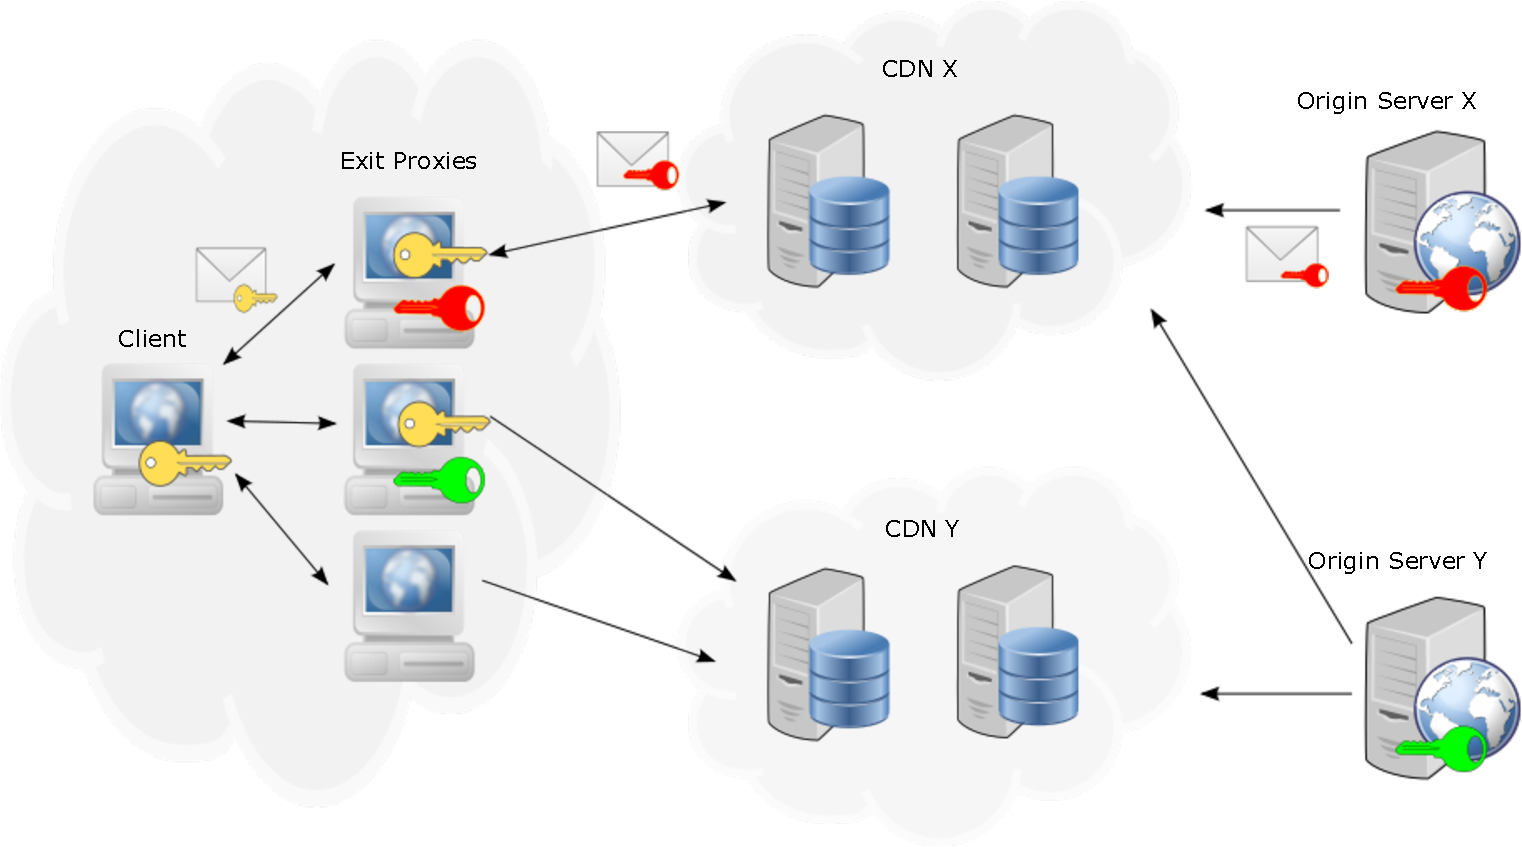
\includegraphics[width=.6\textwidth]{ocdn_overview_updated}
\caption{The relationships between clients, exit proxies, CDNs, and origin servers in 
\system{}.}
\label{fig:ocd_overview}
\end{figure}

\system{} introduces a closed set of proxies (a set of exit proxies).  Using this set of proxies separates the issues of trust and content distribution.  A client no longer needs to trust the CDN, which all other clients would need to trust as well.  Now the client can simply rely on the exit proxies to decouple content distribution from the decision of trust.  

\subsection{Hiding Content}
\label{sec:hiding_content}

We start by discussing how the system components communicate and authenticate one another. 
We introduce shared keys between origin servers and exit proxies, how these keys
are stored, how the exit proxies authenticate themselves to origin servers, and how these 
keys are distributed.

%\begin{table}[t!]
%\footnotesize
%\centering
%\begin{tabular}{ l  p{1.9in} } 
% \multicolumn{1}{c}{\bf Design Decision} & \multicolumn{1}{c}{\bf Function} \\
%\hline \hline
% Shared Keys & {Hides content on cache nodes from CDN.} \\
% Consistent Hashing & {Load balance requests across proxies; ensure no proxy can
% control a given URL.} \\
% Self-Certifying Identifiers & {Authenticates exit proxies to origin servers.} \\
% DNS for Key Sharing & {Allows origin server to share shared keys with exit
% proxies.} \\ \hline
%\end{tabular}
%\caption{Design decisions associated with hiding content from a CDN.}
%\label{tab:setup}
%\end{table}

\textbf{Shared Keys.} 
To prevent an adversary from learning information about content and clients, the CDN must not know anything
about the
content that it is caching.  Therefore, the content {\it and} the associated URL
must be obfuscated
before the CDN sees them.  The content can be obfuscated by encrypting it with a
key that is not
known to the CDN.  Because this must be done prior to caching, the content publisher must 
generate a shared key $k$ to encrypt the content with. Encrypting the content alone does not 
hide all information about content from the CDN; the content identifier, or URL, must also be obfuscated, otherwise the 
CDN can reveal information about which clients accessed which URLs (which is indicative 
of the content).  The obfuscated URL should be fixed and relatively
small; 
these requirements reduce storage requirements and prevent the adversary from guessing
the
URL based on the length of the obfuscated URL.  Unfortunately, using a simple hash allows an 
attacker to guess the content identifier by hashing guesses and comparing with 
the hashes stored in the CDNs caches.  To prevent this attack, the content publisher incorporates the use 
of the shared key $k$ into the hash of the URL by using a hash-based message authentication code 
(HMAC).  Additionally, if the domain supports HTTPS requests, then the content publisher must 
also encrypt the associated certificate with the same key $k$.

The encrypted content and corresponding HMAC are sent to the CDN\footnote{Most CDNs
allow the publisher to
decide on a push or pull model, but \system{} is compatible with either approach.}
and stored in
its caches.  The content publisher then shares the key $k$ with an exit proxy. 
This key allows the 
exit proxy to request encrypted content on behalf of clients by computing the HMAC on the URL.  

\textbf{Consistent Hashing.}
Each exit proxy stores a mapping of URLs to their associated shared key $k$; for example, if 
an origin server has shared key $k$ and publishes a web page {\tt www.foo.com}, then an exit 
proxy will store the mapping of {\tt www.foo.com} to $k$.  The set of exit proxies jointly compute a distributed hash table where the key is the URL ({\tt www.foo.com}) and the value is the 
shared key ($k$).  To assign (key,value) pairs to exit proxies, \system{} uses consistent 
hashing~\cite{karger1997consistent,lewin1998consistent}.  Consistent hashing uses a hash function $H(.)$
to generate identifiers for both exit proxies and for URLs; the identifiers are $H(exit\_ID)$ and $H(URL)$. 
We discuss what $exit\_ID$ is in the next section on Self-Certifying Identifiers.  After the hashes are 
computed, they are mapped to a point on an identifier circle (modulo 2$^{m}$, where $m$ is the length of 
identifier in bits); each URL ($H(URL)$) on the circle is assigned to the first exit proxy ($H(exit\_ID)$) that 
is equal to or follows $H(URL)$ on the circle.  This hashing method is used in \system{} because it provides: 
1)~an evenly distributed mapping of URLs to shared keys among the exit proxies,
2)~a way to prevent an exit 
proxy from choosing which URL it wishes to be responsible for, and 3) a relatively small amount 
of (key,values) to be moved when a new exit proxy is established (or removed).  

\textbf{Self-Certifying Identifiers.} Consistent hashing uses identifiers for both the URLs and 
the exit proxies.  While the identifiers for URLs are straightforward ($H(URL)$), the identifiers for exit 
proxies must provide more information; an exit proxy identifier must be able to prove to an origin server that 
it is the exit proxy that is responsible for the associated URL.  If this validation was not part of \system{}, 
then any (potentially malicious) exit proxy could request the shared key $k$ from any or all origin servers.  To 
prevent a malicious exit proxy from learning any shared key $k$, the proxy must be identified by a self-certifying 
identifer.  This technique was first introduced in a self-certifying file system~\cite{mazieres2000self}; it allows
for other entities (such as origin servers) to certify the exit proxy solely based on its identifier.  The format 
of this identifier ($exit\_ID$) is {\tt IP:hostID}, where {\tt IP} is the exit proxy's IP address and {\tt hostID} 
is a hash of the exit proxy's public key.  A malicious exit proxy cannot \textit{choose} where on the consistent 
hashing ring it sits because it cannot frequently change and re-hash its own IP address (whereas it could re-generate 
a new public key).\footnote{While a malicious exit proxy cannot specifically choose its location on the hashing ring, it 
could recompute a public key until it finds a certain location on the hashing ring.  This is limited by the fact that 
the exit proxy's IP address is part of its identifier, and we assume that the adversary running the exit proxy cannot 
change IP addresses to a value of his choice or in a frequent manner.  A potential attack that an adversary can execute 
on a DHT using a consistent hashing scheme is a Sybil attack, where the adversary runs {\it many} exit proxies to hopefully 
place himself in his desired location on the hashing ring.  We describe countermeasures to a Sybil attack in Section 
\ref{sec:sec}.} When an exit proxy is requesting the shared key $k$ from an origin server, 
it sends its identifier and its public key to the origin server.  The origin server
can then hash the exit proxy's 
public key and verify it against the {\tt hostID}; this action serves as a proof
of the exit proxy's position in the consistent hashing
circle, and thus prevents a proxy from lying about where it lies on the ring (and subsequently lying about which 
URL's shared key it is responsible for).  Note that this $exit\_ID$ is used on the consistent hashing circle as $H(IP):H(hostID)$; the 
$exit\_ID$ must be the same length as $H(URL)$, so the $exit\_ID$ consists of the first half of the bits of $H(IP)$ concatenated 
with the first half of the bits of $H(hostID)$.

\textbf{DNS for Key Distribution.}
We have discussed how shared keys are generated, used, and stored, and here we describe how they are shared.  As previously 
stated, the origin servers generate shared keys and must share them with the (correct) exit proxies.  \system{} uses DNS
to do so.  To retrieve a shared key $k$, an exit proxy sends a DNS query to the origin server's authoritative DNS, and 
it includes its identifier, $exit\_ID$, and its public key in the {\tt Additional Info} section of the query.  The 
authoritative DNS for the origin server validates the exit proxy by hashing the public key and comparing it to the 
second part of $exit\_ID$, and verifying that the exit proxy is responsible for its URL based on the consistent 
hashing circle.  If the verification is successful, then the authoritative DNS sends the shared key $k$ encrypted 
under the exit proxy's public key, \{$k$\}$_{PK_{exit}}$ in the SRV record of the DNS response.  The exit proxy 
extracts $k$ by decrypting with its private key, and stores it in its hash table.

%\begin{table}[t!]
%\footnotesize
%\centering
%\begin{tabular}{ l  p{1.9in} } 
% \multicolumn{1}{c}{\bf Design Decision} & \multicolumn{1}{c}{\bf Function} \\
%\hline \hline
%Spoofed Source Routes & {Hides origin of client request from other
% clients, exit proxies, and CDN.} \\
% Session Keys & {Hides URL and response from other clients.} \\
% Multicast Response & {Allows CDN to return content directly to client without knowing
% the client that requested the content.} \\
% \hline
%\end{tabular}
%\caption{The design decisions associated with content requests and responses, and what these 
%decisions provide.}
%\label{tab:request_response}
%\end{table}

\subsection{Hiding Clients}
\label{sec:hiding_clients}
We make additional design choices that concern the requests that clients initiate
and the responses they receive. We 
introduce session keys for this purpose.

\textbf{Source Routing through Multiple Exit Proxies.}
As previously described, exit proxies query the CDN on behalf of clients, but the
exit proxy
should not be able to learn which client sent which request.  This obfuscation is
accomplished by routing requests through
a series of other exit proxies.  %Each client runs a proxy and is
%also a peer in this system; this 
%peer-to-peer system of clients borrows the 
%protocols used for clients joining, leaving, and learning about other clients from
%the vast literature on peer-to-peer %systems~\cite{monnerat2006d1ht,risson2006stable,zhu2005efficient,gupta2003kelips,lesniewski2008sybil,leong2004achieving}. 
A client routes a request through
intermediate exit proxies by using source routing; when the client generates a request, it also
generates a source route, which includes
the addresses of a set of exit proxies.  The last hop in the source route is the exit proxy that is responsible for the 
shared key $k$ associated with the URL in her request.  The client determines the correct exit proxy by looking up a locally-held URL-proxy map (which is retrieved from a central system that keeps the mapping of URLs to exit proxies).  
It appends this source route to its request and forwards it to the first exit proxy
in the route.  When an intermediate exit proxy receives
a request, she simply forwards it on to the next exit proxy; this continues until the last hop in the source route, which 
is the final exit proxy. 

%To obscure the client that initiated the request, \system{}
%allows each client to spoof source routes; specifically, a client can prepend
%other peers in the route before it initiates a request.  For example, a client
%with identity {\it C} could generate a route to exit proxy {\it E} that looks
%like $C \rightarrow G \rightarrow F \rightarrow E$ and can further obfuscate
%the source of the route by prepending additional clients to the beginning of
%the route as follows: $D \rightarrow A \rightarrow C \rightarrow G \rightarrow
%F \rightarrow E$. Neither {\it G}, {\it F}, nor {\it E} know who the original requestor was; from {\it E}'s point of 
%view, the original requestor could have been {\it D}, {\it A}, {\it C}, {\it G},
%or {\it F}.  Recall from Section \ref{sec:attacker} that our threat model does not 
%include a global passive adversary, and therefore do not prevent an adversary with those capabilities 
%from learning which client issued the request; \system{} does prevent an adversary that is running a 
%client and/or exit proxy from identifying which client issued the request. Using a sequence of 
%peers, or even just knowing that a client {\it can} use a series of peers, hides
%the identity of the client 
%from other clients, exit proxies, and the CDN. 

The option for source routing offers a tradeoff between privacy and performance. Clients interested in prioritizing performance can choose to send requests directly to the correct exit proxy. In such a case, the exit proxy will know the client's identity, but the CDN will not. For more privacy, the client can forward a request through a set of additional exit proxies between it and the final exit proxy. %Lastly, the client could {\it only} prepend other clients' %identifiers but simply %forward the request {\em directly} to the exit proxy; this action provides the same performance benefit as the first mode, but %still offers some %additional privacy benefits. Although the last option would appear to strike the optimal balance between privacy and performance, it %cannot be the only %option because the exit proxy would always know that the true client is the previous hop in the source route. % 
These modes of operation provide clients with different ways to use the system both based on their privacy preferences and the type of content they are requesting.


\textbf{Session Keys for Request and Response Confidentiality.}
In addition to shared keys between origin servers and exit proxies, \system{} uses session keys shared 
between clients and exit proxies.  Session keys provide confidentiality of the requested URL and the 
response.  When the client generates a request, it generates a session key $skey$.
and encrypts 
the URL in her request with this key, which provides \{URL\}$_{skey}$.  The client
must also share this session key
with the exit proxy, so that the exit proxy can learn the plaintext URL and subsequently compute the HMAC to 
query the CDN.  The client encrypts the session key with the exit proxy's public key, resulting in \{skey\}$_{PK_{exit}}$, 
and appends this value as an additional header on the request.  Because her request may be forwarded through a different exit proxy first, this hides the URL of the request from any intermediate exit proxy.

When the last exit proxy receives a request, it first extracts the session
key $skey$ by decrypting it with 
his private key, and then he decrypts the URL with the session key.  This operation
yields the original plaintext
URL. Using the shared key $k$ from the origin server, it can then compute
HMAC$_k$(URL) and forward the request 
to the CDN.  Upon receiving a response from the CDN, the exit proxy then decrypts
the content with the shared key $k$, and
encrypts the content with the session key $skey$ before sending it to the client via the exit proxy that originally forwarded the initial request.
When the client receives the encrypted response, 
she can then decrypt it using $skey$.

%\textbf{Multicast Responses.}
%Using session keys allows for a performance optimization in sending responses back to clients.  Instead of sending 
%the encrypted response from the exit proxy back to the client via the set of peers used in the source route, the exit 
%proxy can send it in a multicast manner to all clients that were on the source route.  The only client that knows $skey$ 
%is the true client that originated the request, therefore none of the other clients can interpret the response, and it reduces the 
%latency for sending the response to the client.  

%\subsection{Incentives for Running \system{}}
%As described in Sections \ref{sec:hiding_content} and \ref{sec:hiding_clients}, \system{} relies 
%on the use of a system of proxies.  These include: 1) client proxies, and 2) exit proxies.  For a client 
%to join the system, they must also run client proxy on his/her machine.  On the other hand, there is no 
%requirement for a client, organization, or company to run an exit proxy; despite this lack of requirement, we 
%believe that both clients and companies have enough incentives to run an exit proxy (or multiple exit proxies).  
%Clients benefit from running an exit proxy because it allows \system{} to perform better in terms of both 
%performance and privacy; when there are more exit proxies, then there is less load put on each exit proxy, and there is a smaller
%chance that an attacker has access to most exit proxies.  Companies benefit from running an exit proxy for similar 
%reasons --- performance and privacy ---, but it could help Internet users access their content quicker (assuming they have 
%content cached by the CDN).    

%\subsection{Incentives}
%While our explanation of the design of \system{} describes a set of proxies that are run by us, but are not 
%trusted; here we describe alternative designs regarding the system of proxies.  The system will work with both a closed, 
%trusted system of proxies, as well as with an open (untrusted) system of proxies.

%{\bf Closed System of Proxies.} While the proxies in \system{} are not trusted, \system{} could 
%use a system of closed and trusted proxies.  There are potential groups or organizations that would 
%support this trusted set of exit proxies, and would be willing (and trusted) to run the exit proxies.  If the exit
%proxies were trusted, then parts of the design of \system{} could be simplified; for example, if proxies 
%were trusted, then \system{} would not need to hide the identity of clients from the exit proxies, and could 
%remove spoofed source routes from the design.  The primary drawback of this approach is finding an organization 
%that everyone could trust to run the exit proxies.  

%{\bf Open System of Proxies.} In \system{}, exit proxies are not 
%trusted with client identities and information, which removes the need to find a universally trustworthy 
%organization.  In an alternative approach, \system{} could use a completely open system of proxies that are 
%untrusted, which would allow anyone (clients, companies, etc.) to run an exit proxy.  
%The addition of an exit proxy follows the protocol in consistent hashing for when a new node 
%joins; some keys would be transferred to the new exit proxy, and clients' mapping of 
%exit proxies will be updated.  This allows for the load to be split among more proxies and 
%increases the geographic diversity of the exit proxies.  

%\subsection{Design Enhancements}

%We discuss possible enhancements to \system{}'s basic design.

%\textbf{Multiple CDNs.}
%While describing the design decisions that went into \system{}, we referred to a single CDN for 
%simplicity.  In reality, \system{} allows for many CDNs to participate;
%distributing content across
%multiple CDNs could provide additional privacy. Origin servers can also take advantage
%of multiple CDNs.

%\textbf{Encoding URLs.}
%As described earlier, each URL is obfuscated by using a HMAC and then stored on the CDN.  An adversary 
%could potentially correlate a URL's popularity with its access patterns.  To prevent this, \system{} allows 
%origin servers to generate multiple different encodings of its URLs, such that HMAC$_k$(enc$_1$(URL)) $\neq$ 
%HMAC$_k$(enc$_2$(URL)).  Each origin server could produce $n$ different encodings of popular URLs, such that 
%the popularity distribution seen by an adversary is a uniform distribution of URL requests across all URLs.  

%\textbf{DHT Replicas.}
%Each exit proxy's hash table can be replicated by another (or many other) exit proxies, spreading the burden across multiple proxies. This behavior would %provide less load per exit proxy, as well as redundancy in case of failures.  Additionally, 
%the CDN can cache the content associated with a given URL at more than one cache
%node;
%if only one exit proxy is responsible for a given URL's content, then it would likely only be cached at 
%cache node closest to the exit proxy.  Having multiple exit proxies responsible for a URL's content 
%helps decrease the load on the proxies while maintaining some of the performance benefits of a CDN.

%\textbf{Hybrid OCDN/CDN Designs.}
%Different origin servers have different needs, and each origin server might 
%have different needs for different content.  The design of \system{} allows origin servers
% to publish some of their content on \system{} and some on other CDNs.  
%This is useful in a case where some content is more sensitive, while other content needs 
%better performance.

%\textbf{Pre-Fetch DNS Responses.} 
%One way to increase the performance of \system{} is to pre-fetch DNS responses at 
%the exit proxies.  This would allow the exit proxy to serve each client request faster 
%because it would not have to send as many DNS requests.  Pre-fetching DNS responses would 
%not take up a large amount of space, but it also would not be a complete set of all DNS 
%responses.  Additionally, if the CDN moves content between cache nodes, then DNS 
%response must also change; therefore, the pre-fetched DNS responses should have a lifetime 
%that is shorter than the lifetime of the content on a cache node.

%\textbf{Privacy vs. Performance Tradeoffs.}
%There are two different modes that \system{} can operate in, where one provides better 
%performance, and the other provides better privacy.  In the first mode, the client can 
%choose to send a request directly to the exit proxy.  
%
%In this case, the exit proxy might be able to discover the identity of the client,
%but the CDN would still not be able to map a request to the client that made the
%request.
%Alternatively, the client can forward a request
%through a set of peers before it reaches the exit proxy.  In this case, the client
%can 
%prepend other clients' identifiers (as previously described) to make it appear as
%though the request came from
%a different client.  This action further obscures the relationship between the client
%and the request.  As another option, the client could {\it only} prepend
%other clients'identifiers but simply forward
%the request {\em directly} to the exit proxy; this action provides the same performance
%benefit as the first
%mode, but still offers some additional privacy benefits.  Although the last option
%would appear to strike the optimal balance between privacy and performance, it cannot
%be
%the only option because the exit proxy would always know that the true client is the previous hop 
%in the source route.  These modes of operation provide clients with different ways to use 
%the system both based on their privacy preferences and the type of content they are requesting.


\section{Evaluation}
\label{sec:eval}

\subsection{Performance Analysis}

\subsection{Security Analysis}

\section{Discussion}
\label{sec:discussion}

In this section, we discuss the various technical, political, and legal limitations
of \system{}, as well as possible avenues for future work. 

\paragraph{\system{} limitations.} CDNs become slightly limited in terms of the 
possible performance optimizations when following \system{}'s design.  For example, 
many CDNs perform HTTPS re-writes on content that they cache, but this can only be 
done if the CDN has access to the decrypted content.  Similarly, the CDN needs the 
decrypted content to perform minimizations on HTML, CSS, and Javascript files.  While 
this likely increases performance in traditional CDNs, it does not provide the greatest 
increase in performance; content caching around the world is the greatest benefit to 
performance, which \system{} preserves.

\paragraph{CDNs operated by content hosts.} The design of \system{}
assumes that the entities operating the proxies and delivering content are
distinct from original content provider. In many cases, however---particularly
for large content providers such as Netflix, Facebook, and Google---the
content provider operates their own CDN cache nodes; in these cases, \system{} will
not be able to obfuscate the content from the CDN operator, since the content host
and the CDN are the same party.  Similarly, because the CDN operator is the same
entity as the original server, it also knows the keys that are shared with the clients.
As a result, the CDN cache nodes could also discover the keys and identify both
the content, as well as which clients are requesting which content.

%\paragraph{Exit proxies run by volunteers.} In the description of \system{} in Sections 
%\ref{sec:design} and \ref{sec:protocol}, we assume we are running the exit proxies, but 
%the design of the system also allows for clients to run exit proxies.  Exit proxies are not 
%trusted with client identities and information, which allows for volunteers to run exit proxies.  
%The addition of an exit proxy follows the protocol in consistent hashing for when a new node 
%joins; some keys would be transferred to the new exit proxy, and clients' mapping of 
%exit proxies will be updated.  This allows for the load to be split among more proxies and 
%increases the geographic diversity of the exit proxies.

%\paragraph{Better mixing with proxy selection} In the current implementation of
%\system{}, a client's requests are all directed through the same \system{} proxy.
%Instead, a client could use a proxy autoconfiguration (PAC) file, which could direct
%requests through different proxies depending on characteristics such as which URL
%is being requested. The selection of proxies might even be randomized.  Randomizing
%the proxy that serves a particular client request ensures that no single proxy knows
%all of the requests that any particular client is making; additionally, it may make
%it more difficult for a CDN to identify the group of requests coming from a single
%client, since a client's requests would mixed among multiple proxies. 

\paragraph{Legal questions and political pushback.} Recent cases surrounding
the Stored Communications Act in the United States raise some questions over
whether a system like \system{} might face legal challenges from law
enforcement agencies. To protect user data against these types of challenges,
Microsoft has already taken steps such as moving user data to data centers in
Germany that are operated by entities outside the United States, such as
T-Systems. It remains to be seen, of course, whether \system{} would face similar
hurdles, but similar systems in the past have faced scrutiny and pushback from law
enforcement.

\section{Related Work}
\label{sec:related}

To our knowledge, there has been no prior work on preventing surveillance at CDNs, but there 
has been relevant research on securing CDNs and finding security vulnerabilities in CDNs.\\
\vspace{0pt}
\textbf{Securing CDNs.} Most prior work on securing CDNs has focused on providing content 
integrity at the CDN as opposed to content confidentiality (and unlinkability).  In 2005, 
Lesniewski-Laas and Kaashoek use SSL-splitting --- a technique 
where the proxy simulates an SSL connection with the client by using authentication records from 
the server with data records from the cache (in the proxy) --- to maintain the 
integrity of content being served by a proxy~\cite{lesniewski2005ssl}.  While this work does not 
explicitly apply SSL-splitting to CDNs, it is a technique that could be used for content 
distribution.  Michalakis et al., present a system for ensuring content integrity for untrusted 
peer-to-peer content delivery networks~\cite{michalakis2007ensuring}.  This system, Repeat and 
Compare, use attestation records and a number of peers act as verifiers.  More recently, Levy et al., 
introduced Stickler, which is a system that allows content publishers to guarantee the end-to-end 
authenticity of their content to users~\cite{levy2015stickler}.  Stickler includes content publishers 
signing their content, and users verifying the signature without having to modify the browser.  Unfortunately, 
systems like Stickler do not protect against an adversary that wishes to learn information about content, clients, 
or publishers; \system{} is complementary to Stickler.\\
%There has been prior work in securing CDNs against DDoS attacks; Gilad 
%et al. introduce a DDoS defense called CDN-on-Demand~\cite{gilad2016cdn}.  In this work they 
%provide a complement to CDNs, as some smaller organizations cannot afford the use of CDNs and 
%therefore do not receive the DDoS protections provided by them.  CDN-on-Demand is a software 
%defense that relies on managing flexible cloud resources as opposed to using a CDN provider's 
%service.\\
\vspace{0pt}
\textbf{Security Issues in CDNs.} More prevalent in the literature than defense are attacks on CDNs.  Liang et al., studied 
20 CDN providers and found that there are many problems with HTTPS practice in CDNs~\cite{liang2014https}.  Some of these 
problems include: invalid certificates, private key sharing, neglected revocation of stale certificates, and 
insecure back-end communications; the authors point out that some of these problems are fundamental issues due to 
the man-in-the-middle characteristic of CDNs.  Similarly, Zolfaghari and Houmansadr found problems with HTTPS usage by 
CDNBrowsing, a system that relies on CDNs for censorship circumvention~\cite{zolfaghari2016practical}.  They found that HTTPS 
leaks the identity of the content being accessed, which defeats the purpose of a censorship circumvention tool. 

Research has also covered other attacks on CDNs, such as flash crowds and denial of service attacks; Jung et al., show 
that some CDNs might not actually provide much defense against flash events (and they differentiate flash events from denial 
of service events)~\cite{jung2002flash}. Su and Kuzmanovic show that some CDNs are more susceptible to intential service 
degradation, despite being known for being resilient to network outages and denial of service attacks~\cite{su2008thinning}. 
Recently, researchers have studied the privacy implications of peer-assisted CDNs; peer-assisted CDNs allow clients to cache and distribute 
content on behalf of a website.  It is starting to be supported by CDNs, such as Akamai, but the design of the paradigm
makes clients susceptible to privacy attacks; one client can infur the cross site browsing patterns of another client~\cite{jia2016anonymity}.
%Additionally, researchers implemented an attack that can affect popular CDNs, such as Akamai and Limelight; this attack 
%defeats CDNs' denial of service protection and actually utilizes the CDN to amplify the attack~\cite{triukose2009content}.  %In the 
%past year, researchers have found forwarding loop attacks that are possible in CDNs, which cause requests to be served repeatedly, which 
%subsequently consumes resources, decreases availability, and could potentially lead to a denial of service attack~\cite{chen2016forwarding}.
%\paragraph{Measuring and Mapping CDNs.} As CDNs have increased in popularity, and are predicted to grow even more~\cite{predict}, much research has 
%studied the deployment of CDNs.  Huang et al., have mapped the locations of servers, and evaluated the server availability for two CDNs: 
%Akamai and Limelight~\cite{huang2008measuring}.  More recently, Calder et al., mapped Google's infrastructure; this included 
%developing techniques for mapping, enumerating the IP addresses of servers, and identifying associations between clients and clusters of 
%servers~\cite{calder2013mapping}. Scott et al., develop a clustering technique to identify the IP footprints of CDN deployments; this analysis
% also analyzes network-level interference to aid in the identification of CDN deployments~\cite{scott2016satellite}.  In 2017, researchers 
%conducted an empirical study of CDN deployment in China; they found that it is significantly different than in other parts of the world 
%due to their unique economic, technical, and regulatory factors~\cite{xue2017cdns}. 
%Other measurement studies on CDNs have focused on characterizing and quantifying flash crowds on CDNs~\cite{wendell2011going}, inferring 
%and using network measurements performed by a large CDN to identify quality Internet paths~\cite{su2009drafting}, and measuring object size distributions and 
%request characteristics to optimize caching policies~\cite{berger2017adaptsize}.

\section{Conclusion}
\label{sec:conclusion}

As more content is distributed via CDNs, CDNs are increasingly becoming the
targets of data requests and liability cases.  We discuss why CDNs are
powerful in terms of the information they know  and can gather, such as a
client's cross site browsing patterns.  In response to  traditional CDNs'
capabilities, we design \system{}, which provides oblivious content
distribution.  \system{} obfuscates data such that the CDN can operate without
having knowledge of  what content they are caching.  This system not only
provides protections to CDNs, but also preserves client privacy by ensuring
that the CDN and the origin server never learn the identity of clients that
make requests for content. \system{} is robust against a strong adversary who
has access to request logs at the CDN and can also join the system as a
client, publisher, or CDN. Our evaluation shows that \system{} imposes some performance
overhead due to the cryptographic operations that allow it to obliviously cache
content, but that this overhead is acceptable, particularly for the sizes of files
that make up common web workloads.
\label{lastpage}

{\footnotesize \bibliographystyle{acm}
\bibliography{paper}}


%\theendnotes

\end{document}







